\chapter{Cinematica}
La cinematica si occupa dello studio geometrico del moto trascurando le cause che lo hanno provocato, le quali invece sono l'oggetto di studio della dinamica del moto.
\begin{figure}[h]
    \centering
    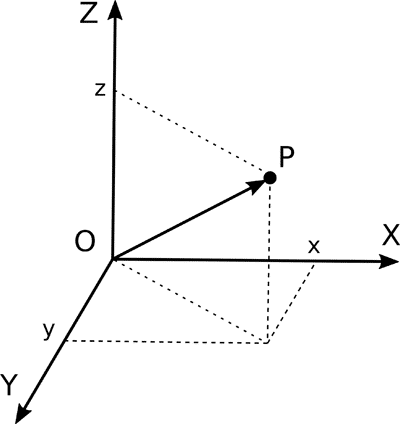
\includegraphics[width=0.3\linewidth]{Immagini/SdR.png}
    \caption{sistema di coordinate cartesiano.}
    \label{fig: SdR}
\end{figure}
Il vettore che unisce i punti $O$ e $P$ si indica con $\vr(t)$, questo permette di calcolare la posizione di $P$ al variare di $t$ sfruttando la scomposizione di $\vr(t)$ lungo gli assi cartesiani
\begin{equation}
    \vr(t)=x(t)\hatu_x+y(t)\hatu_y+z(t)\hatu_z.
\end{equation}
\section{Moto ad una dimensione}
Ci si limita al momento allo studio del moto di corpi puntiformi che si muovono in linea retta.

\begin{defn}[velocità media]
    La velocità media $v_m$ è definita come il rapporto incrementale tra la variazione di posizione e l'intervallo temporale in cui avviene lo spostamento, in formule 
    \begin{equation}
    \label{eq: velocità media}
        v_m=\frac{\Delta x}{\Delta t}=\frac{x_2-x_1}{t_2-t_1}.
    \end{equation}
\end{defn}
Considerando il limite della velocità media $v_m$ si ottiene la velocità istantanea del corpo.
\begin{defn}[velocità istantanea]
    La velocità istantanea $v$ è definita come il limite per $\Delta t\to0$ del rapporto incrementale \eqref{eq: velocità media}, in formule
    \begin{equation}
    \label{eq: velocità istantanea}
        v=\lim_{\Delta t\to0}{\frac{\Delta x}{\Delta t}}=\frac{dx}{dt}.
    \end{equation}
\end{defn}
\begin{obs}
    Considerando l'equazione \eqref{eq: velocità istantanea} e supponendo un moto lungo l'asse $x$, questo avviene nel verso positivo dell'asse se $v>0$ e nel verso negativo se $v<0$.
\end{obs}
A questo punto si è ottenuta una formula della velocità istantanea,
\begin{equation}
    v(t)=\frac{dx}{dt},
\end{equation}
che è a tutti gli effetti un'equazione differenziale risolvibile con il metodo della separazione delle variabili. Quindi si può scrivere
\begin{equation}
    v\,dt=dx.
\end{equation}
Integrando il primo membro tra $t_0$ e $t$ e il secondo tra $x_0$ e $x$ si ottiene
\begin{equation}
    \Delta x=\int_{x_0}^{x}{dx}=\int_{t_0}^{t}{v(t)dt},
\end{equation}
da cui si ricava la legge oraria del moto rettilineo
\begin{equation}\label{eq: legge oraria moto rettilineo}
    x(t)=x_0+\int_{t_0}^{t}{v(t)dt}.
\end{equation}
Analogamente, è possibile definire l'accelerazione media $a_m$.
\begin{defn}[accelerazione media]
    L'accelerazione media $a_m$ è definita come il rapporto incrementale tra la variazione di velocità e l'intervallo temporale in cui avviene questa variazione, in formule 
    \begin{equation}
    \label{eq: accelerazione media}
        a_m=\frac{\Delta v}{\Delta t}=\frac{v(t_2)-v(t_1)}{t_2-t_1}.
    \end{equation}
\end{defn}
Considerando il limite dell'accelerazione media $a_m$ si ottiene l'accelerazione istantanea del corpo.
\begin{defn}[accelerazione istantanea]
    L'accelerazione istantanea $a$ è definita come il limite per $\Delta t\to0$ del rapporto incrementale \eqref{eq: accelerazione media}, in formule
    \begin{equation}
    \label{eq: accelerazione istantanea}
        a=\lim_{\Delta t\to0}{\frac{\Delta v}{\Delta t}}=\frac{dv}{dt}.
    \end{equation}
\end{defn}
\begin{obs}
    Considerando l'equazione \eqref{eq: accelerazione istantanea} e supponendo un moto lungo l'asse $x$, si ha $a>0$ se $v>0$ e $a<0$ se $v<0$.
\end{obs}
A questo punto si è ottenuta una formula dell'accelerazione istantanea,
\begin{equation}
    a(t)=\frac{dv}{dt},
\end{equation}
che è risolvibile nuovamente con il metodo della separazione delle variabili. Quindi si può scrivere
\begin{equation}
    a\,dt=dv.
\end{equation}
Integrando il primo membro tra $t_0$ e $t$ e il secondo tra $v_0$ e $v$ si ottiene
\begin{equation}
    \Delta v=\int_{v_0}^{v(t)}{dv}=\int_{t_0}^{t}{a(t)dt},
\end{equation}
da cui si ricava la formula per la velocità
\begin{equation}
\label{eq: velocità moto rellineo}
    v(t)=v_0+\int_{t_0}^{t}{a(t)dt}.
\end{equation}
Nel caso in cui l'accelerazione $a(t)$ sia una funzione della posizione $a(x)=a(x(t))$ si può scrivere
\begin{equation}
    a=\frac{dv}{dt}=\frac{dv}{dx}\frac{dx}{dt}=v\frac{dv}{dx},
\end{equation}
da cui, usando il metodo di separazione delle variabili, si ottiene
\begin{equation}
    a\,dx=v\,dv.
\end{equation}
Integrando il primo membro tra $x_0$ e $x$ e il secondo tra $v_0$ e $v$ si ottiene
\begin{equation}
    \int_{v_0}^{v}v\,dv=\int_{x_0}^{x}a(x)\,dx,
\end{equation}
da cui
\begin{equation}
\label{eq: v^2 moto rettilineo}
    v^2=v_0^2+2\int_{x_0}^{x}a(x)\,dx.
\end{equation}

\subsection{Moto rettilineo uniforme}
Un corpo si muove di moto rettilineo uniforme (MRU) se si sposta lungo una retta con velocità $v$ costante nel tempo. La legge oraria del MRU si può ricavare dall'equazione \eqref{eq: legge oraria moto rettilineo} considerando appunto $v(t)$ indipendente dal tempo e pertanto ottenendo
\begin{equation}
\label{eq: legge oraria MRU}
    x(t)=x_0+v(t-t_0).
\end{equation}
Ponendo per semplicità $t_0=0$ e $x_0=0$ si ottiene
\begin{equation}
    x(t)=vt.
\end{equation}

\subsection{Moto rettilineo uniformemente accelerato}
Un corpo si muove di moto rettilineo uniformemente accelerato (MRUA) se si sposta lungo una retta con accelerazione $a$ costante nel tempo. La legge oraria del MRUA si può ricavare partendo dall'equazione \eqref{eq: velocità moto rellineo} considerando appunto $a(t)$ indipendente dal tempo e pertanto ottenendo
\begin{equation}\label{eq: v(t) MRU}
    v(t)=v_0+a(t-t_0).
\end{equation}
Si procede ora riconsiderando l'equazione \eqref{eq: legge oraria moto rettilineo} e sostituendo l'equazione \eqref{eq: v(t) MRU} ottenendo
\begin{equation}
    x(t)=x_0+\int_{v_0}^{v}{v_0+a(t-t_0)dt},
\end{equation}
da cui
\begin{equation}\label{legge oraria MRUA}
    x(t)=x_0+v_0(t-t_0)+\frac{1}{2}a(t-t_0)^2.
\end{equation}
Ponendo per semplicità $t_0=0$ e $x_0=0$ si ottiene
\begin{equation}
    x(t)=v_0t+\frac{1}{2}at^2.
\end{equation}
Inoltre, dall'equazione \eqref{eq: v^2 moto rettilineo} si trova
\begin{equation}
    v^2=v_0^2+2a(x-x_0).
\end{equation}

\subsection{Moto armonico semplice}
Un corpo si muove di moto armonico semplice (MAS) se si sposta oscillando con una certa frequenza attorno ad un punto secondo la legge oraria
\begin{equation}
    \label{eq: legge oraria MAS}
    x(t)=A\sin{(\omega t+\phi)},
\end{equation}
dove $\omega$ è la pulsazione e $\phi$ è la fase.
Partendo dall'equazione \eqref{eq: legge oraria MAS} si può ricavare la legge della velocità
\begin{equation}
    \label{eq: v(t) MAS}
    v(t)=\frac{dx(t)}{dt}=\omega A\cos{(\omega t+\phi)}.
\end{equation}
Ponendo $T=t'-t$ e $x(t)=x(t')$ si trova
\begin{equation}
    \omega t'+\phi=\omega t+\phi+2\pi,
\end{equation}
da cui
\begin{equation}
    \omega(t'-t)=\omega T=2\pi,
\end{equation}
dove $T$ è il periodo di oscillazione. Ponendo $t=0$ si trova
\begin{equation}
\label{eq: fase MAS}
    x(0)=A\sin{\phi}\Rightarrow\phi=\arcsin{\left(\frac{x(0)}{A}\right)}.
\end{equation}
Nel caso in cui $\phi=0$ si ha $x(t)=A\sin{\omega t}$, quindi il moto parte dall'origine del sistema di riferimento.

Partendo ora dall'equazione \eqref{eq: v(t) MAS} si può ricavare la legge dell'accelerazione
\begin{equation}
    \label{eq: a(t) MAS}
    a(t)=\frac{dv(t)}{dt}=-A\omega^2\sin{(\omega t+\phi)}=-\omega^2x(t).
\end{equation}
Dall'equazione \eqref{eq: a(t) MAS} si deduce che l'accelerazione è sempre proporzionale allo spostamento, infatti
\begin{equation}
    a(t)=-\omega^2x(t)=\frac{d^2x(t)}{dt^2},
\end{equation}
da cui si ricava l'equazione differenziale di secondo grado del MAS
\begin{equation}
    \label{eq: eq. diff. MAS}
    \frac{d^2x(t)}{dt^2}+\omega^2x(t)=0,\quad x(t)=A\sin{(\omega t+\phi)}.
\end{equation}
Le condizioni al contorno dell'equazione \eqref{eq: eq. diff. MAS} sono per $t=0$
\begin{equation}
    \label{eq: condizioni contorno MAS}
    \begin{cases}
        x_0=A\sin{\phi} \\
        v_0=A\omega\cos{\phi}
    \end{cases}
    \Rightarrow\phi=\arctan{\left(\frac{\omega x_0}{v_0}\right)}.
\end{equation}
Ora dividendo la seconda equazione del sistema \eqref{eq: condizioni contorno MAS} per $\omega$, effettuando il quadrato delle due equazioni e sommandoli si ottiene
\begin{equation}
    A^2=x_0^2+\frac{v_0^2}{\omega^2}.
\end{equation}

\section{Moto in due dimensioni}
La posizione di un corpo in un piano è descritto da un vettore $\vr$ che unisce la posizione del punto all'origine del sistema di riferimento.
\begin{figure}[h]
    \centering
    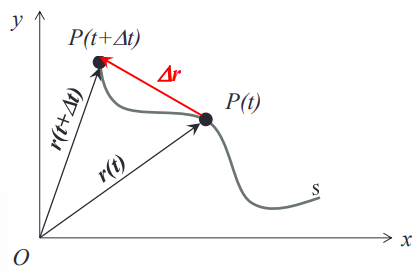
\includegraphics[width=0.5\linewidth]{Immagini/moto in due dimensioni.png}
    \caption{moto in due dimensioni.}
    \label{fig: moto in due dimensioni}
\end{figure}
La velocità istantanea è definita analogamente al caso del moto in una dimensione da
\begin{equation}
\label{eq: velocità moto in due dimensioni}
    \vv=\frac{d\vr}{dt}=\frac{ds}{dt}\hatu_T=v\hatu_T,
\end{equation}
dove $\hatu_T$ è il versore tangente alla traiettoria nel punto $r(t)$. Inoltre, sapendo che $\vr(t)=x(t)\hatu_x+y(t)\hatu_y$, si trova
\begin{equation}
    \vv=\frac{dx}{dt}\hatu_x+\frac{dy}{dt}\hatu_y=v_x\hatu_x+v_y\hatu_y.
\end{equation}
\'E possibile definire la posizione del corpo in coordinate polari, sfruttando l'angolo $\theta(t)$ tra l'asse $x$ e il vettore $\vr(t)$ e il versore radiale $\hatu_r$ parallelo al vettore $\vr(t)$, con cui si può scrivere $\vr(t)=r\hatu_r$. 
\begin{figure}[h]
    \centering
    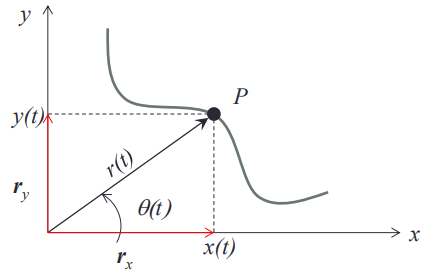
\includegraphics[width=0.55\linewidth]{Immagini/moto in due dimensioni polari.png}
    \caption{moto in due dimensioni in coordinate polari.}
    \label{fig: moto in due dimensioni in coordinate polari}
\end{figure}
La velocità in coordinate polari diventa quindi
\begin{equation}
    \vv=\frac{d\vr}{dt}=\frac{d(r\hatu_r)}{dt}=\frac{d\vr}{dt}\hatu_r+r\frac{d\hatu_r}{dt},\quad\frac{d\hatu_r}{dt}=\frac{d\theta}{dt}\hatu_{\theta}.
\end{equation}
Dunque, la velocità in coordinate polari è data da
\begin{equation}
    \vv=\frac{d\vr}{dt}\hatu_r+r\frac{d\theta}{dt}\hatu_{\theta}=\vv_r+\vv_{\theta},
\end{equation}
dove la prima componente, detta radiale, descrive di quanto si allontana il corpo, mentre la seconda componente, detta trasversa, di quanto esso ruoti.
\begin{figure}[h]
    \centering
    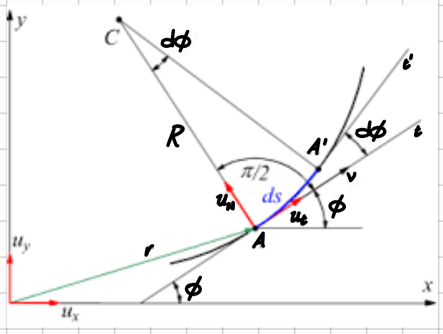
\includegraphics[width=0.6\linewidth]{Immagini/moto 2D diagramma.png}
    \caption{diagramma del moto in due dimensioni in coordinate polari.}
    \label{fig: diagramma del moto in due dimensioni in coordinate polari}
\end{figure}

Conoscendo la legge della velocità si può ricavare la legge dell'accelerazione semplicemente derivando rispetto al tempo l'equazione \eqref{eq: velocità moto in due dimensioni}
\begin{equation}
    \va=\frac{d\vv}{dt}=\frac{d}{dt}(v\hatu_T)=\frac{dv}{dt}\hatu_T+\frac{d\hatu_T}{dt}v,\quad\frac{d\hatu_T}{dt}=\frac{d\varphi}{dt}\hatu_N.
\end{equation}
Dunque, l'accelerazione è data da
\begin{equation}
    \va=\underbrace{\frac{dv}{dt}\hatu_T}_{\substack{\parallel \vv}}+\underbrace{v\frac{d\varphi}{dt}\hatu_N}_{\substack{\perp \vv}}=\va_T+\va_N,
\end{equation}
dove la prima componente esprime la variazione del modulo della velocità, mentre la seconda dipende dalla variazione della direzione di $\vv$, in particolare $\dot{\varphi}$ descrive quanto rapidamente varia la direzione di $\hatu_T$ e quindi di $\hatu_N$. Infine, è possibile riscrivere $\dot{\varphi}$ in funzione di $R$ e $v$. Considerando il differenziale $d\varphi$ si ha
\begin{equation}
    d\varphi=\frac{ds}{R}\Rightarrow\frac{d\varphi}{ds}=\frac{1}{R},
\end{equation}
quindi,
\begin{equation}
    \frac{d\varphi}{dt}=\frac{d\varphi}{ds}\frac{ds}{dt}=\frac{v}{R}.
\end{equation}
Dunque,
\begin{equation}
    \va=\frac{dv}{dt}\hatu_T+\frac{v^2}{R}\hatu_N=\va_T+\va_N.
\end{equation}
\'E possibile distinguere alcuni casi di moto in due dimensioni secondo i valori di $\va_T$ e $\va_N$:
\begin{itemize}
    \item Se $\va_T\neq0$ e $\va_N\neq0$ significa che sta cambiando sia il modulo che la direzione della velocità.
    \item Se $\va_T=0$ e $\va_N\neq0$ significa che il modulo della velocità è costante e varia solo la sua direzione, quindi si ha moto circolare uniforme.
    \item Se $\va_T\neq0$ e $\va_N=0$ significa che la direzione della velocità è costante e varia solo il suo modulo, quindi si ha moto rettilineo vario.
    \item Se $\va_T=0$ e $\va_N=0$ significa che sia il modulo che la direzione della velocità sono costanti, quindi si ha MRU.
\end{itemize}

\subsection{Moto circolare uniforme}
Un corpo si muove di moto circolare uniforme (MCU) se orbita lungo una circonferenza di raggio $R$ a velocità costante. Per studiare questo moto è conveniente usare le coordinate polari
\begin{equation}
    \begin{cases}
        x(t)=R\cos{\theta(t)} \\
        y(t)=R\sin{\theta(t)}
    \end{cases},\quad\theta(t)=\omega t.
\end{equation}
Se il moto non è uniforme allora si hanno
\begin{equation}
    a_T=\frac{dv}{dt},\quad\omega=\frac{v}{R},\quad\alpha=\frac{d\omega}{dt}=\frac{a_T}{R}.
\end{equation}
Dunque, sapendo che $\theta=S/R$ e se $\vv=\vom\times\vr$, si ha
\begin{equation}
    \begin{split}
        \va&=\frac{d\vv}{dt}=\frac{d}{dt}(\vom\times\vr)=\frac{d\vom}{dt}\times\vr+\frac{d\vr}{dt}\times\vom \\
        &=\alpha\times\vr+\vom\times\frac{d\vr}{dt}=\va_T+\va_N.
    \end{split}
\end{equation}
\begin{obs}
    La pulsazione $\omega$ in generale può essere una funzione del tempo anche rispetto alla direzione, in tal caso la legge continua ad essere valida cambiando l'asse di rotazione.
\end{obs}

\subsection{Moto parabolico}
Un corpo si muove di moto parabolico se, partendo con una certa velocità iniziale $v_0$ e un certo angolo $\theta$, percorre una traiettoria sotto l'azione della sola forza di gravità.
\begin{figure}[h]
    \centering
    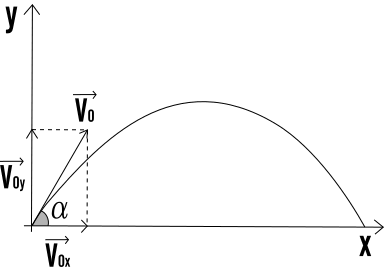
\includegraphics[width=0.4\linewidth]{Immagini/moto parabolico.png}
    \caption{diagramma del moto parabolico.}
    \label{fig: moto parabolico}
\end{figure}
L'accelerazione di gravità è $\va=-g\hatu_y$, la velocità iniziale si scompone lungo gli assi cartesiani come $\vv_0=v_{0x}\hatu_x+v_{0y}\hatu_y$, dove $v_{0x}=v_0\cos{\theta}$ e $v_{0y}=v_0\sin{\theta}$. Quindi, la velocità è data da
\begin{equation}
    \vv=\vv_0+\int_0^t\va(t)\,dt=\vv_0-gt\hatu_y.
\end{equation}
La posizione del corpo è data da
\begin{equation}
    \vr(r)=\vr_0(t)+\int_0^t\vv(t)\,dt=\vv_0t-\frac{1}{2}gt^2\hatu_y=v_{0x}t\hatu_x+(v_{0y}-\frac{1}{2}gt^2)\hatu_y.
\end{equation}
Quindi, le leggi orarie dei moti proiettati sono
\begin{equation}
    \begin{cases}
        x(t)=v_{0x}t \\
        y(t)=v_{0y}t-\dfrac{1}{2}gt^2
    \end{cases}.
\end{equation}
Dalla prima equazione si ricava il tempo $t$ come
\begin{equation}
    t=\frac{x}{v_{0x}}=\frac{x}{v_0\cos{\theta}},
\end{equation}
che sostituito nell'equazione di $y(t)$ restituisce la traiettoria del corpo
\begin{equation}
    y(x)=v_0\sin{\theta}\frac{x}{v_0\cos{\theta}}-\dfrac{1}{2}g\bigg(\frac{x}{v_0\cos{\theta}}\bigg)^2=x\tan{\theta}-\frac{g}{2v_0^2\cos^2{\theta}}x^2.
\end{equation}